
\documentclass[conference]{IEEEtran}
\usepackage{blindtext}
\usepackage{graphicx}
\usepackage{tabulary}
%\usepackage{tikz}
\usepackage{pgfplots}
\usepackage[simplified]{pgf-umlcd}
\usepackage{listings}
\usepackage{array}
\usepackage[left=1.2cm,right=1.2cm,top=2cm,bottom=2cm]{geometry}
\graphicspath{ {images/} }
\lstdefinestyle{customhtml}{
  language=HTML,
  showstringspaces=false,
  basicstyle=\scriptsize\ttfamily,
  keywordstyle=\bfseries\color{green!40!black},
  commentstyle=\itshape\color{purple!40!black},
  identifierstyle=\color{blue},
  stringstyle=\color{orange},
  tabsize=2
}

\definecolor{javared}{rgb}{0.6,0,0} % for strings
\definecolor{javagreen}{rgb}{0.25,0.5,0.35} % comments
\definecolor{javapurple}{rgb}{0.5,0,0.35} % keywords
\definecolor{javadocblue}{rgb}{0.25,0.35,0.75} % javadoc
\definecolor{javaStringBlue}{rgb}{0.1647,0,1}

\lstdefinestyle{customjava}{
language=Java,
basicstyle=\scriptsize\ttfamily,
keywordstyle=\color{javapurple}\bfseries,
stringstyle=\color{javaStringBlue},
commentstyle=\color{javagreen},
morecomment=[s][\color{javadocblue}]{/**}{*/},
tabsize=4,
showspaces=false,
showstringspaces=false
}

\ifCLASSINFOpdf
  % \usepackage[pdftex]{graphicx}
  % declare the path(s) where your graphic files are
  % \graphicspath{{../pdf/}{../jpeg/}}
  % and their extensions so you won't have to specify these with
  % every instance of \includegraphics
  % \DeclareGraphicsExtensions{.pdf,.jpeg,.png}
\else
  % or other class option (dvipsone, dvipdf, if not using dvips). graphicx
  % will default to the driver specified in the system graphics.cfg if no
  % driver is specified.
  % \usepackage[dvips]{graphicx}
  % declare the path(s) where your graphic files are
  % \graphicspath{{../eps/}}
  % and their extensions so you won't have to specify these with
  % every instance of \includegraphics
  % \DeclareGraphicsExtensions{.eps}
\fi

\begin{document}
%
% paper title
% can use linebreaks \\ within to get better formatting as desired
\title{Collaborative Platform for Analysis of Software Systems}


% author names and affiliations
% use a multiple column layout for up to three different
% affiliations
\author{\IEEEauthorblockN{Catarina Isabel Carvalho Santana}
\IEEEauthorblockA{Instituto Superior T\'{e}cnico\\
Email: catarina.santana@tecnico.ulisboa.pt}}

% make the title area
\maketitle


\begin{abstract}
The Software Architectures course at Instituto Superior T\'{e}cnico teaches students the most important concepts on design and architecture of software systems and helps students to apply these concepts to real and complex software systems. Organizing knowledge and applying theory to practice is not an easy task, and students often need to ask questions and discuss. State-of-the-art on collaborative, social software and knowledge structuring was analyzed and a social platform was developed to help solving these problems.
\end{abstract}

% Note that keywords are not normally used for peerreview papers.
\begin{IEEEkeywords}
social software, knowledge structuring, collaborative platform, reputation systems, tagging systems, ontology, taxonomy.
\end{IEEEkeywords}

\section{Introduction}
\label{introduction}
Analyzing and discussing big, real, open-source and highly complex software system is a very important part of the Software Architectures course at Instituto Superior T\'{e}cnico. In the course context, students must apply concepts and techniques for design and analysis of software architectures to descriptions of real systems. However, applying these concepts and techniques is not a very easy task, and often students have questions and doubts regarding these descriptions. These questions sometimes require not only consulting the course bibliography, but also discussing with peers or asking questions to teachers. This thesis focuses on providing a solution for this problem with the use of social software and knowledge structuring strategies.

This document is organized as follows: Section \ref{problemDescription} gives a more detailed description about the problem of applying theoretical concepts to practical examples in the context of the Software Architectures course. Section \ref{objectives} elicits the main goals of this thesis. Section \ref{relatedWork} presents the state-of-the-art in the areas of Social Software and Knowledge Structuring. Section \ref{solution} gives a small description of the developed solution. Sections \ref{domainModel}, \ref{architecture} and \ref{implementation} describe the solution domain model, architectural details and implementation. Finally, Section \ref{evaluation} will show the assessment of the developed solution and \ref{futureWork} will describe what can still be added to it.

\section{Problem Description}
\label{problemDescription}
The course of Software Architectures teaches students the most important concepts in the field of software architectures and applies these concepts to real-life software systems. In the practical component of this course, software description articles are analyzed to identify the theoretical concepts in practical examples. This analysis is either done by students with the help of the teacher, during practical classes, or in work groups where they read, discuss and analyze software descriptions together and present their results to both the teacher and the rest of the class.

Understanding the analysis done and how it was done is very important, since it means students can apply the concepts learned not only in the written exam to pass the course, but also in the future, in other real-life software systems. However, there are several issues regarding the application of theory concepts in this course:
\begin{itemize}
\item The course has around one-hundred students per year. Each person is different, and while some students may quickly understand what is taught in theory lessons, others may need some more time to assimilate what was taught.

\item The output of the analysis done to software descriptions (the scenarios, etc. extracted) is not available in a consistent way for everyone, it is usually limited to the student's individual notes or the work done in groups.

\item The case description is usually a fairly long document, and correlating the concepts learned in theory classes with the practical examples is not easy, as the parts of the text that map to concepts are not always evident.

\item The architectural elements extracted from a single software description are usually scattered along the whole text, and it is not evident the connection between all the elements.
\end{itemize}

\section{Objectives}
\label{objectives}
To solve the problems mentioned in Section \ref{problemDescription}, a collaborative platform was planned and developed, where students and teachers collaborate in the analysis and synthesis of the case descriptions, ending on a structured representation of the case descriptions, that is hooked on the concrete description. 

The goal of the platform is to provide ways for annotating the text on the case descriptions, which will help students organizing their thoughts and creating the structure, and use elements of social software, as a way of promoting collaboration, mutual aid, learning and even some competition between students.
 
The existence of this collaborative should provide not only a way for students to discuss, ask questions and consolidate their knowledge, but also a unique place where their study materials are stored and organized, facilitating their studies.

\section{Related Work}
\label{relatedWork}
The platform to develop can be thought of a social software, where different people communicate and collaborate to provide a structured representation of a software description.
The next sections provide an overview on the state-of-the-art of two main aspects:
\begin{itemize}
\item \textbf{Collaborative work}, presenting the state-of-the-art on social and collaborative aspects of software. This includes literature on the \textbf{Honeycomb Framework}, a framework that generalizes the most important components of social software, \textbf{Persuasive Software}, systems that have impact on users behavior and thoughts, which is the case of the platform to develop, \textbf{Roles in Social Networks}, describing the types of users of social software and \textbf{Reputation Systems}, which is the attribution of scores to users to provide a motivational component on the platform.
	
\item \textbf{Knowledge Structuring}, presenting the state-of-the-art on ways of structuring information. This includes literature on \textbf{Collaborative tagging }systems, which consists of assigning keywords to documents or parts of documents, \textbf{Semi-structured content}, which consists of providing a way for structuring knowledge without such strict rules as, for example, an ontology or a taxonomy and \textbf{Ontology Learning}, extracting knowledge from text.
\end{itemize}

\subsection{Honeycomb Framework}
\label{relatedWorkHoneycomb}
The definition of Social Software as ``systems that allow people, in their particularities and diversity, to communicate (interact, collaborate, exchange ideas and information) mediating and facilitating any kind of social relationship and favoring the emergence of a collective wisdom and a bottom-up organization'' \cite{pereira2010social} applies to our collaborative platform, as it should allow students with different personalities and opinions to participate by identifying architectural elements, asking questions, etc. in order to reach a complete and correct analysis of that system. 

The Honeycomb Framework was proposed to illustrate the seven elements that give a functional definition for social software \cite{smith2007social}: \textbf{Identity}, the unique identifier of a user within the system, which applies to the platform to develop in the sense that each student is a unique person and must have a unique identification in the platform; \textbf{Presence}, resources that allow knowing if certain identity is online, which are not strictly necessary in the platform; \textbf{Relationship}, way to determine how users can relate/are related to others, which applies to the platform as students are related to each other both as colleagues as and group elements, and to the teachers; \textbf{Reputation}, way of knowing the status of a user in the system, which could be used to assess the quality and relevance of the contributions to the platform; \textbf{Groups}, possibility to form communities of users that have common interests, which applies to the platform as students form work groups; \textbf{Conversation}, resources for communication among the users (synchronous and/or asynchronous). In the context of the platform, conversation should be done asynchronously with comments and discussions; \textbf{Sharing}, possibility of sharing objects that are important to the users (videos, images, etc), which applies to this context as students may want to share documentation or other media with their colleagues or their group;

\subsection{Persuasive Software Design Patterns}
\label{relatedWorkPersuasive}
The term ``persuasive technology'' is used to describe computer systems that have an impact on user's thoughts and may even lead to changes in their behavior \cite{fogg2002persuasive,oinas2009persuasive}.

There are three different possible outcomes for a persuasive system: \textbf{Reinforcement}, making current attitudes resistant to change, \textbf{Changing Outcome }, changes in a person's response to an issue, and \textbf{Shaping Outcome}, formulate a pattern for a situation where one did not exist before \cite{oinas2008towards}. The most important outcome for this platform is the Changing Outcome: When a description of a system is presented, the students most not only read it, but also relate it to the concepts learned and use the platform to try and extract the correct scenarios and views from it.

The concept of social influence describes a change in one's behavior (or attitudes or beliefs), caused by external pressures \cite{guadagno2010preference}. In our context, students may not contribute to the platform at first, but may feel compelled to when seeing their colleagues' contributions. Four design patterns are proposed for persuasive systems, in order to introduce social influence in software features: Social Learning and Facilitation (SLF), Competition (COM), Cooperation (COO) and Recognition (REC) \cite{oduor2014persuasive}. 

The \textbf{Social Learning and Facilitation} pattern has the main purpose of using software features that allow to visualize the presence of other people, with the motivation that it is easier for individuals to pursue their goals if there is a clear awareness of other people pursuing the same goal and facing the same issues \cite{oduor2014persuasive}. In the context of our collaborative platform, students may not contribute at first, but may feel compelled to as they see their colleagues contributing.

The \textbf{Competition} pattern has the main purpose of using competitive elements, such as ranks, scores and levels, that allow users to compare their performance with others, and adjust their target goals based on these. Some people may see this competition as a source of anxiety, so participation must be voluntary \cite{oduor2014persuasive}. Adding a score for each student and a rank hierarchy based on the range of scores will start a hopefully healthy competition between them. Anonymity should be an option in the platform, to remove sources of anxiety.

The \textbf{Cooperation} pattern has the main purpose of providing software features that allow users to engage in mutual goals and support each other. The motivation for this pattern is that it is easier to cooperate if people are engaged in mutual objectives. However, some people prefer to perform alone, so cooperation must not be forced \cite{oduor2014persuasive}. The students in the platform will be working towards a main goal: correctly understanding and correlating what was learned in the Software Architectures classes with real examples of software systems. But there are several concepts and structures to identify on a single description and students may have difficulties in identifying them, so dividing the main goal in several smaller goals and have discussions around them would be useful.

The \textbf{Recognition} pattern has the purpose of providing software features that enable users to get recognition from their peers. The motivation for this pattern is that users sometimes need a reason to focus on reaching their goals. Having their efforts recognized may be a good reason to keep the good work\cite{oduor2014persuasive}. As the system should have a score system, it could be used as a way of creating a weekly top ten of the students who achieved most points in that week. Recognition is then achieved when students see their names highlighted.

\subsection{Roles in Social Networks}
A \textit{role}, in a social structure, is a set of expectations for an individual in a certain position. For example, the role of ``secretary'' is associated to what secretaries are expected to do \cite{forestier2012roles,nadel1957theory}. There are two categories of roles: \textit{Non-explicit roles}, which are not defined a-priori but can be inferred, and \textit{Explicit roles}, which are predefined types of actors in the social network, such as ``experts'' or ``influencers''.

In the platform to develop, it is possible to define a priori the two main roles: the \textbf{Students}, which are the most active users in the platform as they contribute to the analysis of the software descriptions, and the \textbf{Teachers} which corresponds to a very small number of users in the platform. Their number of contributions is smaller and they are mostly for adding correction to the contents added by the students to the platform.

\subsection{Reputation Systems}
\label{relatedWorkRepsys}
Reputation systems are of extreme importance for certain kinds of applications, namely e-commerce websites, where money transactions are executed and the reputation of a seller will denote the degree of trust that possible buyers will have in them \cite{vavilis2014reference}.

For the platform to develop, reputation does not play such an important role, but will add a motivational component to the platform: Students rate their colleagues' contributions and should try to get and keep a high reputation score. The motivation behind the importance of including a reputation system in the platform is the study conducted \cite{dencheva2011dynamic}, concerning the lack of participation in Moknowpedia, a Wiki system. A reputation system was added to the wiki in order to solve these problems and improve both content quality and quantity\cite{prause2008approach}, and results showed an increase of 62\% in the number of article revisions and an increase of 42\% in the number of viewed articles.
	
\subsubsection{Requirements and Features of the Reputation System}

A framework for analysis of reputation systems is proposed in \cite{vavilis2014reference}, where the general requirements for reputation systems are elicited and the corresponding features needed for their fulfillment. Given the context of the platform, its reputation system requires that \textbf{Ratings and Reputation should discriminate user behavior}, as these scores should allow to identify students with few and/or less relevant contributions and students with many and/or very relevant ones, \textbf{the reputation system should be able to discriminate ``incorrect'' ratings}, as malicious users are present everywhere and can give intentionally inaccurate ratings, \textbf{Users should not be able to modify ratings, reputation values and calculate their own reputation}, as this data should not be accessible to them, and the score should be calculated by the reputation system.

To satisfy the identified requirements, the reputation system should feature a range of values to represent \textbf{trust and distrust}, where low values indicate students with few and/or less relevant contributions and high values indicate students with many and/or very relevant ones, \textbf{absolute reputation values}, calculated independently for each user, and identification of \textbf{origin and target} of the ratings, to prevent self-ratings and identify potential malicious users

\subsubsection{Components of a Reputation System}
Reputation systems are divided in four components\cite{liu2012systematic,liu2010evaluation}, and each have a set of defined criteria for their evaluation: \textbf{Input}, the process of collecting reputation information from information sources, \textbf{Processing}, the procedure of computing and aggregating the reputation information, \textbf{Output}, the dissemination of the reputation information and the \textbf{Feedback Loop}, the collection of feedback of the output (review of the review), which does not apply to the context of the platform.

Concerning the \textbf{Input} component, ratings are collected in the platform and are given by the students that are logged in. Only a single property is collected, the rating assigned.Concerning the \textbf{Processing} component, a weighted average algorithm is the best choice to aggregate ratings in this simple system, and information should be updated as soon as the ratings are assigned. Both the algorithm and the system have a very low complexity. Concerning the \textbf{Output} component, the end users of the information are the students registered in the platform, and this information is only available inside the platform. The reputation information consists in the result of the weighted average algorithm.

\subsection{Collaborative Tagging}
Collaborative tagging is the practice of allowing anyone to freely attach keywords or tags to content \cite{golder2006usage}. Tagging-based systems contrast with taxonomies as they are neither exclusive nor hierarchical, and allow to identify content as being about a great variety of things simultaneously \cite{golder2006usage}. The tags added to content may describe the content itself, or describe the category in which the content falls \cite{coates2005two}. It is possible to identify several functions for the tags, within the system that uses the tagging system \cite{golder2006usage}.

In this platform we are aiming for using tags from a closed taxonomy as a way of identifying the main parts of a software system within a software description, namely stakeholders, scenarios and their parts, tactics, etc., and use the tagged text to create a structured description of the document.

\subsection{Semi-Structured Content}
Knowledge can be obtained from many different resources, ranging from unstructured (for example, language models obtained from plain text) to structured ones (for example, ontologies) \cite{hovy2013collaboratively}. However, unstructured resources do not allow for complex inference chains\cite{domingos2007toward} and information is not ontologized\cite{hovy2013collaboratively}, and structured resources require a huge amount of effort to create and maintain\cite{hovy2013collaboratively}. Semi-structured contents try to create a middle-ground between these two types. The most important example of their use is the Wikipedia, which is a repository of web pages, related with each other by links. Massive online collaboration allow for updated high quality and wide coverage of contents. To sum up, using semi-structured resources provides the best of both worlds: high quality information with wide coverage of almost all domains \cite{hovy2013collaboratively}.
 
The main goal of this platform is to allow students to extract a semi-structured representation of a software system from a description in plain text, and have all the parts that constitute a software system described in a structure similar to a Wikipedia, instead of scattered along a ten or more pages article. This will be accomplished by creating templates for the concepts and associating information from the document to them. Student collaboration in the platform will lead to good quality structured descriptions of the articles.
	
\subsection{Ontology Learning}
Research on Ontology learning from text has evolved over the years and there are several open challenges for this field \cite{wong2012ontology}. Ontologies are defined as ``effectively formal and explicit specifications in the form of concepts and relations of shared conceptualizations'' \cite{gruber1993translation}, and can be thought of as a directed graph, with concepts as nodes and relations as edges. Techniques for ontology learning can be classified in statistics-based, linguistics-based, logic-based or hybrid.

Regarding the context of the platform, all the concepts used to tag the document contents (the concepts of Software Architectures) and their will be defined a priori. Software description documents do not contain these concepts, but the students' motivation is to find parts of the text that correspond to the concepts predefined and tag them accordingly. This facilitates the comprehension of the text contents and the creation of the semi-structure as mentioned previously.

\section{Solution}
\label{solution}
To solve the problems elicited throughout this document, it was developed a Web Application to be used by students and teachers, both in class and home environments. This kind of application facilitates collaboration between its users, and therefore was the more adequate choice for the system to develop. The developed application features an \textbf{authentication system}, where users can login into the system, \textbf{document management}, only available for teachers, where software description articles can be added or removed, \textbf{document parsing } into a view, creation of \textbf{annotations} in the document text, which are parts of selected text annotated with tags, and \textbf{templates }for a set of Software Architectures concepts, which aggregate the corresponding annotations and describe the concepts.

The next sections will give an overview of the domain, and explain the architecture and implementation of the system.
\section{Domain Model}
\label{domainModel}
To understand the architectural and implementation decisions taken during the solution development, it is necessary to understand the Software Architectures Domain Model. Section \ref{domainModel:SAConcepts} lists and describes the concepts talked in the Software Architectures classes, Section \ref{domainModel:Model} presents an abstract domain model where it is possible to see how these concepts relate and Section \ref{domainModel:templates} gives an idea on how the information from the domain model can be represented in templates.

\subsection{Concepts}
\label{domainModel:SAConcepts}
Before describing the domain model of the developed solution, it is necessary to provide a small introduction to the most important concepts from the Software Architectures course.

A \textbf{Scenario} is used to capture and express the quality requirements of a system. The considered qualities are \textbf{Availability}, \textbf{Interoperability}, \textbf{Modifiability}, \textbf{Performance}, \textbf{Security}, \textbf{Testability} and \textbf{Usability}.

A scenario consists of six parts\cite{bass2003software}: The \textbf{Source of Stimulus}, \textbf{Stimulus}, \textbf{Environment}, \textbf{Artifact}, \textbf{Response} and \textbf{Response Measure}. Each Scenario uses a set of \textbf{Tactics}, which achieve the quality requirements. Each quality requirement has a set of commonly used tactics.

A \textbf{View} is a representation of a set of system elements and the relationships associated with them \cite{clements2003documenting}. This set of elements and relationships is constrained by viewtypes, which define the element types and relationship types used to describe the architecture of a software system from a particular perspective. Viewtypes refine into styles, which are specializations of element and relation types, together with a set of constraints on how they can be used. Views can fall into three viewtype categories: The \textbf{Module Viewtype}, which documents the system principal units of implementation, the \textbf{Component \& Connector Viewtype}, which documents the system units of execution, and the \textbf{Allocation Viewtype}, which documents the relationships between a system's software and its development and execution environments. 

\subsection{Model}
\label{domainModel:Model}
Figure \ref{figure:abstractDomainModel} shows the concepts and relations described in Section \ref{domainModel:SAConcepts} in a Domain Model Diagram.
\begin{figure}[ht]
\centering
\renewcommand {\umltextcolor}{black}
\renewcommand {\umlfillcolor}{none}
\renewcommand {\umldrawcolor}{black}

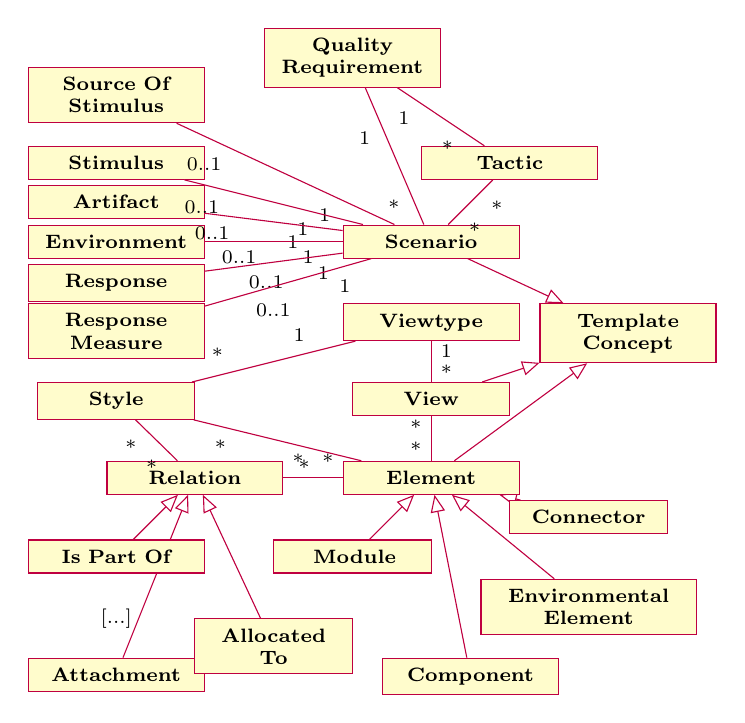
\begin{tikzpicture}
\tikzstyle{every node}=[font=\scriptsize]
\begin{class}[text width=2cm]{Template Concept}{2.5,-3.5}
\end{class}

\begin{class}[text width=2cm ]{Source Of Stimulus}{-4, -0.5}

\end{class}
\begin{class}[text width=2cm ]{Stimulus}{-4,-1.5}
%\inherit{ScenarioElement}
\end{class}
\begin{class}[text width=2cm ]{Artifact}{-4,-2}
%\inherit{ScenarioElement}
\end{class}
\begin{class}[text width=2cm ]{Environment}{-4,-2.5}
%\inherit{ScenarioElement}
\end{class}
\begin{class}[text width=2cm ]{Response}{-4,-3}
%\inherit{ScenarioElement}
\end{class}
\begin{class}[text width=2cm ]{Response Measure}{-4	,-3.5}
\end{class}
\begin{class}[text width=2cm ]{Scenario}{0,-2.5}
\inherit{Template Concept}
\end{class}
\begin{class}[text width=2cm ]{Quality Requirement}{-1,0}
\end{class}
\begin{class}[text width=2cm ]{Tactic}{1,-1.5}
\end{class}

\begin{class}[text width=1cm ]{View}{0,-4.5}
\inherit{Template Concept}
\end{class}
\begin{class}[text width=2cm ]{Viewtype}{0,-3.5}
\end{class}
\begin{class}[text width=1cm ]{Style}{-4,-4.5}
\end{class}
\begin{class}[text width=2cm ]{Relation}{-3,-5.5}
\end{class}

\begin{class}[text width=2cm ]{Element}{0,-5.5}
\inherit{Template Concept}
\end{class}

\begin{class}[text width=2cm]{Is Part Of}{-4,-6.5}
\inherit{Relation}
\end{class}

\draw [umlcd style] (-4,-7.5) node {[...]};

\begin{class}[text width=2cm]{Attachment}{-4,-8}
\inherit{Relation}
\end{class}

\begin{class}[text width=1.5cm]{Allocated To}{-2,-7.5}
\inherit{Relation}
\end{class}

\begin{class}[text width=1cm]{Module}{-1,-6.5}
\inherit{Element}
\end{class}

\begin{class}[text width=2cm]{Component}{0.5,-8}
\inherit{Element}
\end{class}

\begin{class}[text width=2.5cm]{Environmental Element}{2,-7}
\inherit{Element}
\end{class}

\begin{class}[text width=1.5cm]{Connector}{2,-6}
\inherit{Element}
\end{class}

\association{Source Of Stimulus}{}{0..1}{Scenario}{}{1}
\association{Stimulus}{}{0..1}{Scenario}{}{1}
\association{Artifact}{}{0..1}{Scenario}{}{1}
\association{Environment}{}{0..1}{Scenario}{}{1}
\association{Response}{}{0..1}{Scenario}{}{1}
\association{Response Measure}{}{0..1}{Scenario}{}{1}
\association{Quality Requirement}{}{1}{Scenario}{}{*}
\association{Quality Requirement}{}{1}{Tactic}{}{*}
\association{Scenario}{}{*}{Tactic}{}{*}
\association{View}{}{*}{Viewtype}{}{1}
\association{Viewtype}{}{1}{Style}{}{*}
\association{Style}{}{*}{Element}{}{*}
\association{Style}{}{*}{Relation}{}{*}
\association{View}{}{*}{Element}{}{*}
\association{Element}{}{*}{Relation}{}{*}
\end{tikzpicture}
\caption{Domain Model showing the Software Architectures concepts and how they are related}
\label{figure:abstractDomainModel}
\end{figure}
The scenario elements are associated to the Scenario, and each Scenario captures a single Quality Requirement and has a set of Tactics. A View is associated with a Viewtype, which refines into a style. The View contains a set of elements, which have relations with each other. The Scenario, View and Elements are considered the main concepts of the domain, and they have a dedicated template in the developed solution. These templates will contain information about the concept and how it is related with other concepts in the domain model.

\subsection{Templates}
\label{domainModel:templates}
The structured representation of the Software Architectures concepts described in Sections \ref{domainModel:SAConcepts} and \ref{domainModel:Model} is represented in the developed solution by using specific templates for these concepts. It did not make sense to have a template for each concept, as it is easier to see how they relate if they are in the same template, for example, it is easier to see the Scenario elements if they are inside the Scenario template. Figure \ref{figure:scenarioTemplate} shows a Schema example for the Scenario template. All the Scenario elements, the quality requirement and the tactics are present in the template.

\begin{figure}
\centering
\lstinputlisting[language=HTML, style=customhtml]{scenarioSchema.html}
\caption{Schema for the Scenario template}
\label{figure:scenarioTemplate}
\end{figure}

The templates for the View and View Elements follow the same idea of the Scenario schema. The template for the elements represents the element information and also its relations with other elements. The View template has the particularity that, besides including information about the view, also includes the templates of the elements present in it.

\section{Architecture Analysis}
\label{architecture}
Section \ref{domainModel} introduced the domain model of the Software Architectures concepts present in the developed solution, and the templates in which they are included. In this section, it is shown how these templates are filled with information extracted from a software description article. The next subsections will present two main entities from the system: the Document and the Annotation.

\subsection{Document}
\label{architecture:Document}

The Document entity in this system corresponds to a software system description article. Figure \ref{figure:documentEntity} shows the Document entity in the system.
\begin{figure}[ht]
\centering
\renewcommand {\umltextcolor}{black}
\renewcommand {\umlfillcolor}{none}
\renewcommand {\umldrawcolor}{black}

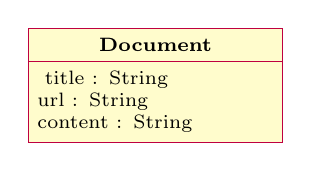
\begin{tikzpicture}
\tikzstyle{every node}=[font=\scriptsize]
\begin{class}[text width=3cm ]{Document}{0,0}
	\attribute { title : String }
	\attribute { url : String }
	\attribute { content : String }
\end{class}
\end{tikzpicture}
\caption{The Document Entity}
\label{figure:documentEntity}
\end{figure}

As the main purpose of this application is to create a structured representation of the document using the templates described in Section \ref{domainModel:templates}, the instances of the main concepts are associated with the Document.  

\subsection{Annotation}
\label{architecture:annotation}

An annotation is a portion of text from the article, enriched with a tag. Figure \ref{figure:annotationEntity} shows the Annotation entity in the system. The ``annotation'' field saves a JSON representation of the annotation data.
\begin{figure}[ht]
\centering
\renewcommand {\umltextcolor}{black}
\renewcommand {\umlfillcolor}{none}
\renewcommand {\umldrawcolor}{black}

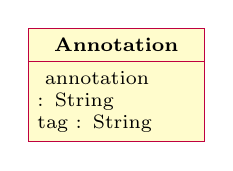
\begin{tikzpicture}
\tikzstyle{every node}=[font=\scriptsize]
\begin{class}[text width=2cm ]{Annotation}{0,0}
	\attribute { annotation : String }
	\attribute { tag : String }
\end{class}
\end{tikzpicture}
\caption{The Annotation Entity}
\label{figure:annotationEntity}
\end{figure}
Annotations are added to the system by selecting a portion of text in the parsed document and setting it as an annotation. Therefore, they are always associated to the Document in which they were created and, as they describe partially or totally a Software Architectures concept, can be associated not only with the main concepts, but with all the concept entities of the domain model. 

\subsection{Interface Flow}
\label{section:interfaceFlow}

The associations between the entities described in the previous sections are created after a set of interactions with the system. These interactions are the creation of an annotation by using the AnnotatorJS interface, the association of that annotation to a domain concept and the redirection to that concept template, where annotations can be moved or deleted and other information, including description text, can be added.

\section{Implementation}
\label{implementation}
The application developed follows a Model-View-Controller architecture. The next sections will describe the solution implementation based on these three elements.

\subsection{Model}
\label{implementation:model}
The Model of the implemented system is based on the Domain Model from Section \ref{domainModel} and the domain model is specified in the Domain Modeling Language, which was created for the F\'{e}nix Framework\cite{cachopo2006combining,cachopo2007development}.

Regarding \textbf{Annotations}, similarly to what is described in \ref{architecture:annotation}, in the implemented model Annotations are associated with the Document in which they were created, and to the User that created it.

\textbf{Scenarios} are represented in the implemented model in a very similar way to what is shown in Figure \ref{figure:abstractDomainModel}. However, the Quality Requirement is not associated with the Tactic, as the set of Quality Requirements and Tactics are not predefined in the implemented database, they are added upon Scenario creation. The Scenario is associated with the respective Document and the Annotations that describe it. Scenario elements are also associated with their respective annotations.

The \textbf{Modules} are the elements of the Module Viewtype Views. The Module entity in the implemented domain model is associated with the corresponding document upon its creation, and with the set of Annotations that describe it, as described in Section \ref{architecture}.

Modules are related to each others, as seen in Figure \ref{figure:abstractDomainModel}. Instead of defining these relations in a separate entity, they are represented in the implemented model with different associations from the Module entity to itself, as seen in Figure \ref{figure:modelIsPartOfRelation}.

\begin{figure}
\centering
\lstset{style=customjava}
\begin{lstlisting}
relation moduleIsPartOfModule {
	Module playsRole parent{ multiplicity 0..1; }
	
	Module playsRole child{ multiplicity 0..*; }
}
\end{lstlisting}
\caption{Is-Part-Of relation between Modules in the implemented model}
\label{figure:modelIsPartOfRelation}
\end{figure}

\textbf{Components and Connectors} are the elements of the Component \& Connector Viewtype Views. A Component has a set of Ports, and a Connector as a set of Roles. Figure \ref{figure:modelComponentConnector} shows how the Components, Connectors and their respective Ports and Roles are implemented.
\begin{figure}
\centering
\renewcommand {\umltextcolor}{black}
\renewcommand {\umlfillcolor}{none}
\renewcommand {\umldrawcolor}{black}
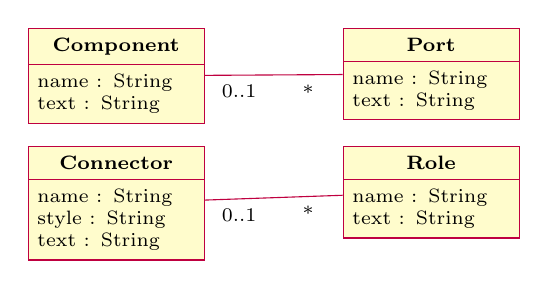
\begin{tikzpicture}
\tikzstyle{every node}=[font=\scriptsize]
\begin{class}[text width=2cm ]{Component}{0,0}
	\attribute {name : String}
	\attribute {text : String}
\end{class}

\begin{class}[text width=2cm ]{Connector}{0,-1.5}
	\attribute {name : String}
	\attribute {style : String}
	\attribute {text : String}
\end{class}

\begin{class}[text width=2cm ]{Port}{4,0}	
	\attribute {name : String}
	\attribute {text : String}
\end{class}

\begin{class}[text width=2cm ]{Role}{4,-1.5}
	\attribute {name : String}
	\attribute {text : String}
\end{class}

\association{Component}{}{0..1}{Port}{}{*}
\association{Connector}{}{0..1}{Role}{}{*}
\end{tikzpicture}
\caption{Component and Connector entities in the implemented model}
\label{figure:modelComponentConnector}
\end{figure}

The Component and Connector are main concepts of the system, and therefore are associated with the corresponding document upon creation. Both the Component and Connector entities and also the Port and Role are associated to a set of Annotations that describe them.

Components are related with Connectors by the \textit{Attachment} relation, in which Component ports are attached to roles of Connectors. The \textit{Attachment} relation was defined by creating an association between the Port and Role entities, as shown in Figure \ref{figure:modelAttachmentRelation}.

\begin{figure}
\lstset{style=customjava}
\begin{lstlisting}
relation portIsAttachedToRole {
	Port playsRole port { multiplicity 0..1; }
	
	Role playsRole role { multiplicity 0..1; }
}
\end{lstlisting}
\caption{Attachment relation between Component Ports and Connector Roles in the implemented model}
\label{figure:modelAttachmentRelation}
\end{figure}

Regarding \textbf{Views}, a View is considered a main concept, and therefore has its own dedicated template. Figure \ref{figure:modelView} shows how it is represented in the implemented model.

\begin{figure}
\centering
\renewcommand {\umltextcolor}{black}
\renewcommand {\umlfillcolor}{none}
\renewcommand {\umldrawcolor}{black}
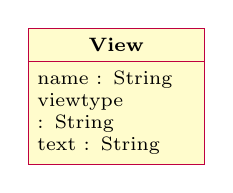
\begin{tikzpicture}
\tikzstyle{every node}=[font=\scriptsize]
\begin{class}[text width=2cm ]{View}{0,0}
	\attribute {name : String}
	\attribute {viewtype : String}
	\attribute {text : String}
\end{class}
\end{tikzpicture}
\caption{View entity in the implemented model}
\label{figure:modelView}
\end{figure}

The viewtype of a View is defined upon its creation and stored in the ``viewtype'' attribute, and the styles of a view are not explicitly stated, but they are implicit by the elements that are added to it. A View is composed by a set of Elements, as seen in Figure \ref{figure:abstractDomainModel}. In the implemented domain model, the View has a similar association with the Module, Component and Connector entities. Figure \ref{figure:modelviewelements} exemplifies the association with the Module entity in the Domain Modeling Language.

\begin{figure}
\lstset{style=customjava}
\begin{lstlisting}
relation viewHasModules {
	View playsRole view { multiplicity 0..*; }
	Module playsRole module { multiplicity 0..*;}
}
\end{lstlisting}
\caption{Relation between View and the view elements}
\label{figure:modelviewelements}
\end{figure}

A View is created by associating an Annotation with it and, as it is a main concept, it is associated with the respective Document.

\subsection{Controller}

This section describes the Controller part of the implemented system. The application developed uses the Spring\footnote{https://spring.io/} Framework, which allows the definition of one or more Java classes to act as Controllers and handle requests.

The \textbf{AnnotationController} class provides a way to manage the annotations added to a document. It communicates with the Domain Model to create, remove or update Annotations. This controller is in fact a RestController, which means it provides a REST API, used to retrieve a JSON representation of the annotations stored in the model and display it along with the document text. 
The endpoints provided by this controller are described in Table \ref{table:endpoints}.
\begin{table}[ht]
\scriptsize
\centering
\begin{tabular}{ | m{1cm} | c | m{2cm} |m{4cm}|}
    \hline
    \textbf{Name} & \parbox[c][0.8cm]{1cm}{\textbf{Request}\\\textbf{Method }}& \textbf{Endpoint} & \textbf{Description}\\ \hline
	INDEX & GET & \parbox[c][0.8cm]{3.5cm}{/selectDoc/\{docId\}/\\store/annotations} & \parbox[c]{8cm}{Returns the set of annotations associated\\with the document with id \textit{docId} }\\ \hline
   	READ & GET & \parbox[c][0.8cm]{3.5cm}{/selectDoc/\{docId\}/\\store/annotations/\{id\}} & Returns the annotation with the specific \textit{id} \\ \hline
    CREATE & POST & \parbox[c]{4cm}{/selectDoc/\{docId\}/\\store/annotations} & \parbox[c][1.5cm]{8cm}{Creates a new annotation, stores it in the \\model associated with the document with\\id \textit{docId}, and redirects to the READ\\endpoint} \\ \hline
    UPDATE & PUT & \parbox[c][0.8cm]{3.5cm}{/selectDoc/\{docId\}/\\store/annotations/\{id\}} & \parbox[c]{8cm}{Updates the annotation with the given \textit{id}\\and redirects to the READ endpoint} \\ \hline
    DELETE & DELETE & \parbox[t]{3.5cm}{/selectDoc/\{docId\}/\\store/annotations/\{id\}} & \parbox[c][1.5cm]{8cm}{Removes the association between the \\ annotation with the given id and the\\document with id \textit{docId}. The response is\\a HTTP/1.0 204 NO CONTENT.} \\ \hline
  \end{tabular}
\\
\caption{REST API provided by the Annotation Controller}
 \label{table:endpoints}
\end{table}

The \textbf{DocumentController} class handles the requests to view, add or remove a document from the system.

Adding and removing documents from the system is a feature that only Teachers are authorized to use. 
To add a new document, the controller checks if the database already contains a document with the given URL and then extracts the article contents from that URL to add to the database. When a teacher removes a Document from the system, all Annotations and Domain Model entities associated with that Document such as Scenarios or Views are removed from the system as well.

Upon Document visualization, there are other operations handled by this controller, such as redirecting operations to other controllers upon receiving a request to visualize the template of a concept or to associate annotations with domain entities as seen in Figure \ref{figure:documentControllerLinkAnnotation}, and navigation to the page containing the structured representation of the document.

\begin{figure}
\lstset{style=customjava, basicstyle=\tiny}
\begin{lstlisting}
	@RequestMapping(value = "/addAnnotationToStructure/{docId}/{annotationId}/{tag}")
	public RedirectView addAnnotationModal(@PathVariable String docId,
			@PathVariable String annotationId, @PathVariable String tag) {
		RedirectView rv = null;
		if (Utils.allScenarioConcepts().contains(tag)) {
			rv= new RedirectView("/addAnnotationToScenarioStructure/" + docId + "/"
					+ annotationId);
		} else if (tag.contains("Module")) {
			rv = new RedirectView("/addAnnotationToModuleTemplate/" + docId + "/"
					+ annotationId);
		}else if (tag.contains("View")) {
			rv = new RedirectView("/addAnnotationToViewTemplate/" + docId + "/"
					+ annotationId);
		}else if (tag.contains("Component")) {
			rv = new RedirectView("/addAnnotationToComponentTemplate/" + docId + "/"
					+ annotationId);
		}else if (tag.contains("Connector")) {
			rv = new RedirectView("/addAnnotationToConnectorTemplate/" + docId + "/"
					+ annotationId);
		}
		return rv;
	}	
\end{lstlisting}
\caption{Redirecting requests to associate annotations with domain entities in the DocumentController}
\label{figure:documentControllerLinkAnnotation}
\end{figure}

The \textbf{ScenarioController} provides means to add and remove Scenarios from the document and link or unlink annotations from a Scenario or its elements.A Scenario is created when a user wants to link an Annotation to a Scenario and is prompted the interface to add a new or choose an existing one. When the Controller receives the request to add a new Scenario, it does not only adds a new Scenario to the database, but also adds a new SrcOfStimulus, Stimulus, Artifact, Environment, Response and ResponseMeasure to the database, all associated with the newly created Scenario. 


When the user chooses which Scenario to link the Annotation with, the controller verifies the tag associated with the Annotation, and add the Annotation either to the Scenario or to the corresponding element. 

A Scenario is initially created without any tactics. Upon receiving the corresponding request, the controller adds a new ``Tactic'' to the database, associated with the corresponding Scenario. Inside the template, annotations can be associated with the specific tactics. 

When user text is added to a Scenario or one of its elements, a request is sent to this Controller. It will then update the Model accordingly and show the updated Model in the corresponding View.

Similarly to the Scenario Controller, the \textbf{ModuleController} handles the creation and deletion of Modules. It also handles the linkage of Annotations to existent Modules and the addition of user text to a Module. The implementation of the methods that handle these operations is similar to the implementation done in the Scenario Controller.

As Modules are related to each other, the Module Controller handles adding and removing other Modules to/from the possible relations. The modules to associate are selected within the template. 

The \textbf{ComponentController} and \textbf{ConnectorController} classes handle the creation and deletion of Components and Connectors from the system. The two classes have very similar methods.

A Component has a set of Ports, which can be attached to Connector Roles. Adding and removing Ports to a component is very similar to the methods implemented to adding and removing tactics from a Scenario. Initially a Component has no Ports, and these can be created inside the Component template. The implementation of the Connector Roles is similar to the implementation of the Ports.

As mentioned in Section \ref{implementation:model}, component ports can be associated with the connector roles by a relation of \textit{attachment}. Inside a Component template, it is possible to attach each of the ports to a Role from an existent Connector.

The \textbf{ViewController} class handles the creation and deletion of Views from two possible Viewtypes: Module and Component \& Connector. 

Similar to the other domain entities, a new View is created when the user wants to associate an annotation with the tag ``View'' with a domain entity.
The ViewController distinguishes between two different templates when receiving a request to view the View's template: One for Module Viewtype views and one for the Component \& Connector Viewtype views, to which only Components and Connectors can be added.
 
When, inside the template, the user selects a set of Modules, Components or Connectors to add to a view, a request is sent to the ViewController, which handles the association of these elements with the respective view.

\subsection{Views}
\label{section:Views}
This section describes how the information from the Model is displayed to the user. The developed application uses Thymeleaf\footnote{http://www.thymeleaf.org/}, a Java template engine for displaying dynamic templates.

Thymeleaf allows the definition of template fragments, which are pieces of code that can be defined in a separate file and be included in any template as desired. Fragments are used in the developed application in the page header, which is included in all templates, and in the concept templates. Figure \ref{figure:viewsHeaderFragment} shows how a fragment is defined. Each fragment must have a unique name and all HTML code of that fragment is then defined inside the \textit{section} tags.
\begin{figure}
\lstset{style=customhtml}
\begin{lstlisting}
<section layout:fragment="headerFragment">
	<nav class="navbar navbar-inverse" id="headernavbar">
		Header definition here	
	</nav>
</section>
\end{lstlisting}
\caption{Defining the Header fragment in Thymeleaf syntax}
\label{figure:viewsHeaderFragment}
\end{figure}

Including a predefined fragment in a template is as easy as Figure \ref{figure:viewsIncludeFragment} shows.
\begin{figure}
\lstset{style=customhtml}
\begin{lstlisting}
<section layout:include="@{/headerFragment} :: headerFragment">
</section>
\end{lstlisting}
\caption{Including a fragment in Thymeleaf syntax}
\label{figure:viewsIncludeFragment}
\end{figure}

The templates use the information added by the Controllers to the Model Attributes and display it in a structured way. This information is actually Java objects from the Model. Thymeleaf allows to treat these attributes as Java objects, so it is possible to obtain the value of the class attributes, or call methods on that object. For example, in Figure \ref{figure:viewsCallingMethods}, the quality requirement and the name of a Scenario object are accessed.

\begin{figure}
\lstset{style=customhtml}
\begin{lstlisting}
<span th:text="'Scenario for '+
	${scenario.getQualityRequirement().getName()}
	+ ': '">
</span> 
<span th:text="${scenario.getName()}"></span>
\end{lstlisting}
\caption{How Thymeleaf accesses variables}
\label{figure:viewsCallingMethods}
\end{figure}

Thymeleaf also provides automatic binding of forms information to provided objects. For example, Figure \ref{figure:viewsModalFormExample} shows a form with checkboxes, to select Modules.
\begin{figure}
\centering
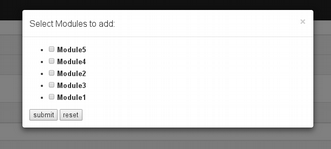
\includegraphics[scale=0.7]{/modalExample}
\caption{Example of a Modal window containing a form}
\label{figure:viewsModalFormExample}
\end{figure}

When the form is submitted, Thymeleaf will bind the selected values to an object passed, and send that object in the body of the POST request to the Controller.

\section{Evaluation}
\label{evaluation}
The success of a software system is often dependent on the opinion of the people that will use it. Systems attractive and easy to use according to the target audience background are more likely to be highly used.

The developed system tries to make the task of reading, understanding and structuring a software description article into an easy one, providing a simple and clean interface.

As the main goal of the developed application is to be used by students and teachers, in both classroom and home environments, it was asked to the students enrolled in the Software Architectures course to test the application, namely the features for annotating text and structuring Scenarios from the annotations created.

The participating students were asked to fill a small survey afterwards to register their opinions.
This survey consisted of a grid question to evaluate aspects of the application usability in a scale from one to ten, three questions asking to evaluate the usefulness of the application in a scale of one to ten, and three open and optional questions, asking what did the student like the most about the application, what improvements could be done to it, and to register any other feedback the student may had.

A total of eight students volunteered to test the application. From these eight, five answered the survey. Due to the small number of participants and little feedback, the results shown are merely indicative, as it is impossible to take valuable conclusions from such a small sample.

Regarding the usability of the application, Figure \ref{figure:usabilityEvaluation} shows the graph containing the ratings given by the students.

\begin{figure}[h]
\centering
\begin{normalsize}
\textbf{Usability of the Application's Features}\\
\end{normalsize}
\scriptsize
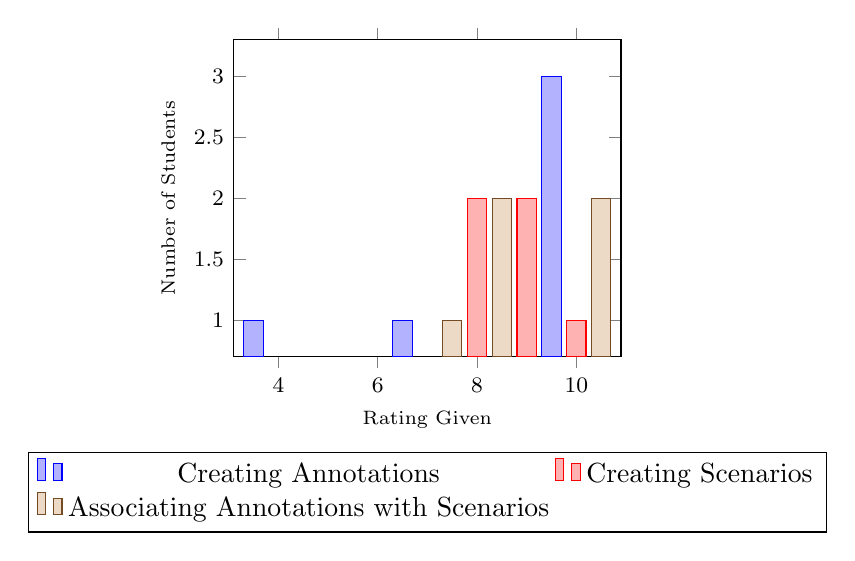
\begin{tikzpicture}
\begin{axis}[
small,
x tick label style={
/pgf/number format/1000 sep=},
ylabel=Number of Students,
ylabel style={font=\scriptsize},
xlabel=Rating Given,
xlabel style={font=\scriptsize},
enlargelimits=0.15,
legend style={at={(0.5,-0.3)},
anchor=north,legend columns=2},
ybar,
bar width=7pt,
]
\addplot 
	coordinates {(7,1) (4,1) (10,3)};
\addplot 
	coordinates {(9,2) (10,1) (8,2)};
\addplot
	coordinates {(8,2) (10,2) (7,1)};	
\legend{Creating Annotations, Creating Scenarios, Associating Annotations with Scenarios}
\end{axis}
\end{tikzpicture}
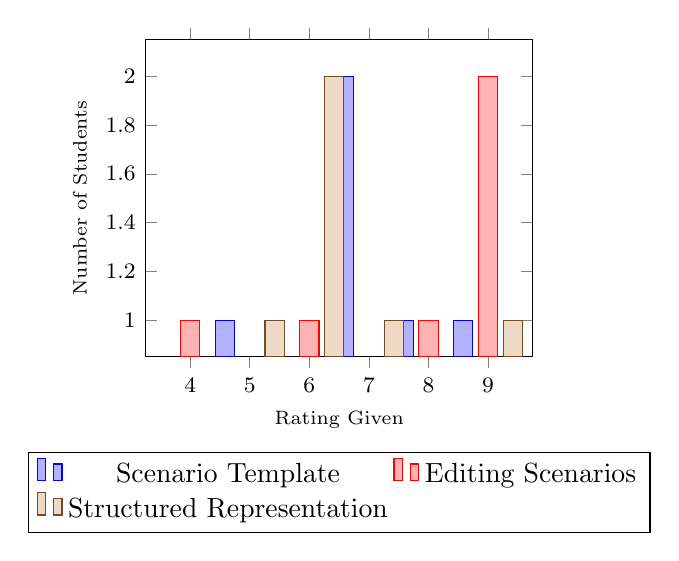
\begin{tikzpicture}
\begin{axis}[
small,
x tick label style={
/pgf/number format/1000 sep=},
ylabel=Number of Students,
ylabel style={font=\scriptsize},
xlabel=Rating Given,
xlabel style={font=\scriptsize},
enlargelimits=0.15,
legend style={at={(0.5,-0.3)},
anchor=north,legend columns=2},
ybar,
bar width=7pt,
]

\addplot
	coordinates {(5,1) (7,2) (9,1) (8,1)};
\addplot
	coordinates {(4,1) (6,1) (9,2) (8,1)};
\addplot
	coordinates {(5,1) (6,2) (9,1) (7,1)};  	
\legend{Scenario Template, Editing Scenarios, Structured Representation}
\end{axis}
\end{tikzpicture}
\caption{Evaluation results regarding the usability of the application}
\label{figure:usabilityEvaluation}
\end{figure}

Overall students thought the application is easy to use regarding creating Scenarios and associating annotations with them. However, there were complaints about the AnnotatorJS interface, such as \textit{``I had trouble when trying annotate a sequence of letters when that sequence overlapped with another annotation''}, which implies that it is not very intuitive when trying to create multiple annotations in the same piece of text.

Improvements suggested in the survey include \textit{``There should be a way to ``view'' the scenario itself, with the diagram that is showed in the lectures. Also, the system needs to be more intuitive, particularly when it comes to selecting sentences for the scenarios''} and \textit{``Make multiple copies of the article to be only seen by each group so that one group doesn't get confused or get influenced by others.''}. This reinforces the idea that the AnnotatorJS interface is not very intuitive sometimes, and the need of creating groups in the platform, which is explained in \ref{futureWork}.

When asked what did they like the most about the application, students pointed that \textit{``It is possible for different people to analyze the same document, and its easy to use''} and \textit{``It provides a quick and convenient way of constructing scenarios''}. These opinions help conclude that the platform satisfies the requirement of providing collaboration among students, and facilitates understanding the Software Architectures concepts.

Regarding the usefulness of the application, the survey asked to rate how much the application facilitates the application of theoretical concepts to practical examples, and how useful would it be in the context of the Group Assignments and Practical Classes. Figure \ref{figure:usefulnessEvaluation}

\begin{figure}[h]
\centering
\begin{normalsize}
\textbf{Application Usefulness}\\
\end{normalsize}
\scriptsize
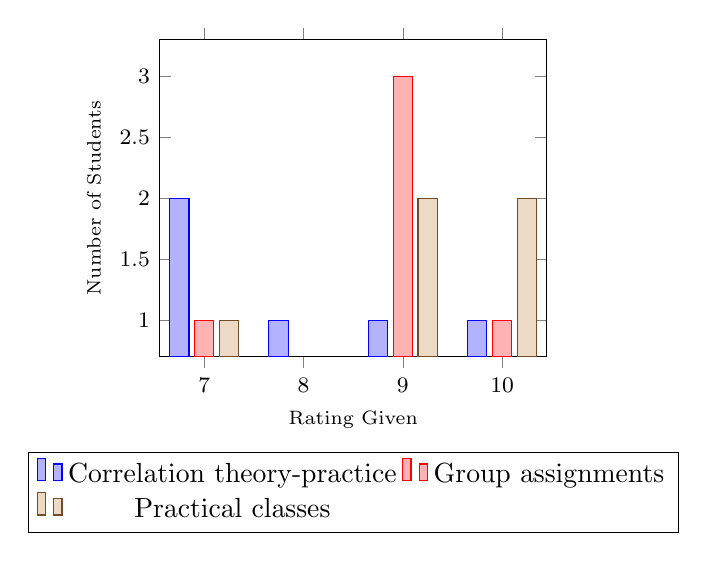
\begin{tikzpicture}
\begin{axis}[
small,
x tick label style={
/pgf/number format/1000 sep=},
ylabel=Number of Students,
ylabel style={font=\scriptsize},
xlabel=Rating Given,
xlabel style={font=\scriptsize},
enlargelimits=0.15,
legend style={at={(0.5,-0.3)},
anchor=north,legend columns=2},
ybar,
bar width=7pt,
]
\addplot 
	coordinates {(7,2) (8,1) (9,1) (10,1)};
\addplot 
	coordinates {(9,3) (7,1) (10,1)};
\addplot
	coordinates {(7,1) (9,2) (10,2)};	
\legend{Correlation theory-practice, Group assignments, Practical classes}
\end{axis}
\end{tikzpicture}
\caption{Evaluation of the usefulness of the application}
\label{figure:usefulnessEvaluation}
\end{figure}

Overall, students would like to use this application for both their Group Assignments and when discussing a description article in the Practical classes. 

In conclusion, the evaluation of the platform, despite the small number of testers, provided positive feedback. The platform proved to provide collaboration, and students appreciated how the information from the text can be extracted into a single template. 

\section{Future Work}
\label{futureWork}
Developing a platform that provides structuring knowledge from an unstructured source and all the described social features was a very ambitious goal for the time span available. 

The developed solution focused on the association of tags from a closed vocabulary to parts of text, and the creation of a semi-structured representation of the software description articles, which was the most important goal of this thesis.

There are still details of the developed solution that could be improved and new features that could be added in the future.

\subsection{Allocation Viewtype}
Allocation viewtype elements should be added to the platform in a future version, so Allocation Viewtype Views can be added to the structured representation of the article.

\subsection{Graphical Representation of Views}
It is easier to understand Views in a graphical representation, and it would be very useful for the platform to provide a way to create or upload these representations in the future

\subsection{Social Elements}
Sections \ref{relatedWorkHoneycomb}, \ref{relatedWorkPersuasive} and  \ref{relatedWorkRepsys} list a series of social features that could be useful in the platform.

The developed platform contains social elements and allows for collaboration, as students are individually identified within the system and work together over a shared article. However, there are several other social software elements that could enrich the platform as a social system, such as \textbf{Groups}, so students can work on their group assignments, \textbf{Discussion Forums} to provide communication and cooperation, a \textbf{Reputation System} to motivate students to contribute, and a \textbf{Spotlight} with the students with highest reputation scores, to provide recognition of their efforts.

\section{Conclusions}
The success of social software is very dependent on the people that use it, since it is focused on the interactions and collaboration between their users.

Developing a platform including not only a way to structure knowledge but also a set of social features is a very ambitious task, and the focus of this thesis was the knowledge structuring part, which is very important for the context of the Software Architectures course.

Although the main feature of the developed solution is the possibility of extracting structured information from an unstructured source, this is done by a set of users authenticated within the system, which can collaboratively read and work over the same text.

Despite its simplicity and the lack of volunteers to test it, overall the platform proved that it provides a way for students to work together. However, there are still many features that could be added to make it more collaborative and more social.

\bibliographystyle{IEEEtran}  
\bibliography{mybib}  

% that's all folks
\end{document}


